%!TeX spellcheck = en-US,en-DE

\begin{frame}{Some properties of Fermi gas}
  Particles dwell in a large but finite volume $\mathcal{V}$.\\
  Periodical boundary conditions.\\
  Restriction on values of the wave vector:

  \begin{equation}
    \veck = 2 \pi \left ( \frac{n_x}{L_x},  \frac{n_y}{L_y}, \frac{n_z}{L_z} \right)
  \end{equation}

  The volume of the unit cell in k-space:

  \begin{equation}
    d\valk_x d\valk_y d\valk_z = d^3\valk = \frac{(2 \pi)^3}{\mathcal{V}}
  \end{equation}
\end{frame}

\begin{frame}[t]{Some properties of Fermi gas}
  \vspace{0.5cm}
  Particles occupy all energy levels bellow Fermi energy.
  Volume in k-space:

  \begin{equation}
    V_\valk = \frac{4}{3}\pi \valk_F^3
  \end{equation}

  \only<1>{
    \begin{figure}
      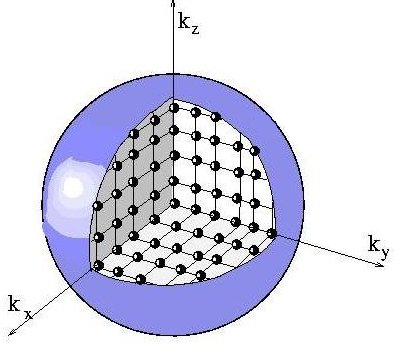
\includegraphics[height=4cm]{fsphere}
      %\caption{}
      \label{fsphere}
    \end{figure}
  }
  \only<2>{
    Number of particles:
    \begin{equation}
      \begin{gathered}
        N = g_{\sigma}\frac{V_\valk}{d^3\valk} = \frac{2\frac{4}{3}\pi \valk_F^3 \mathcal{V}}{8 \pi^3} =
        \frac{\valk_F^3 \mathcal{V}}{3 \pi^2} \implies \\
        \valk_F^3 = \frac{3 \pi^2 N}{\V}
      \end{gathered}
    \end{equation}
  }
\end{frame}

\begin{frame}{Fermionic ground state}
  In the ground state $\ket{g}$ fermions occupy all available
  levels in the k-space up to $\valk_F$:
  \begin{figure}
    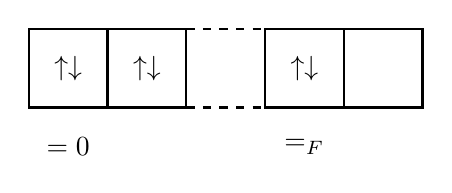
\begin{tikzpicture}
      \foreach \xbox in {0, ..., 1} {
        \def\ybox{0}
        \node at (\xbox+0.5,\ybox+0.5) {$\uparrow \downarrow$};
        \path[draw,thick] (\xbox,\ybox) rectangle (\xbox+1,\ybox+1);
      }
      \node at (0+0.5,0-0.5) {$\valk = 0$};
      \path[draw,dashed,thick] (2,0) -- (3,0) (2,1) -- (3,1);
      \def\xbox{3}
      \node at (\xbox+0.5,0+0.5) {$\uparrow \downarrow$};
      \path[draw,thick] (\xbox,0) rectangle (\xbox+1,0+1);
      \node at (\xbox+0.5,0-0.5) {$\valk = \valk_F$};
      \def\xbox{4}
      \path[draw,thick] (\xbox,0) rectangle (\xbox+1,0+1);
    \end{tikzpicture}
    %\caption{}
    %\label{}
  \end{figure}
\end{frame}
